% \noindent
% \textcolor{red}{
% Dúvidas e Pendências:
% \begin{itemize}
%     \item TODO: Padronizar as Tabelas e Figuras em Português ou Inglês?
%     \item TODO: \textit{Screenshots} da DIO no Estudo de Caso 1: Videoaulas com Legendadas?
%     \item TODO: Retomar as Hipóteses e QPs nos Resultados dos Estudos de Caso ou na Conclusão?
% \end{itemize}
% }

A crescente demanda por ambientes educacionais mais inclusivos evidencia a importância da TA para promover o acesso igualitário à educação, independentemente das barreiras sensoriais, cognitivas ou físicas que os aprendizes possam enfrentar. Dentre essas barreiras, destaca-se a falta de acessibilidade de OAs audíveis para pessoas com deficiência auditiva, o que exige soluções tecnológicas que garantam uma experiência educacional mais inclusiva.

A \autoref{chapter5-phd-synthesis}, apresentada a seguir, sintetiza o percurso metodológico desta pesquisa, conectando os objetivos, métodos e principais resultados obtidos. Neste contexto, o presente trabalho de doutorado discutiu o desenvolvimento e a avaliação da arquitetura \textit{Speech2Learning}, cujo principal objetivo é ampliar a acessibilidade de OAs audíveis, abrangendo, mas não se limitando, à comunidade de aprendizes que utilizam línguas de sinais, como a Libras. A arquitetura foi avaliada por meio da integração de tecnologias de ASR e recursos de TA, como avatares de Libras, visando à criação de soluções flexíveis e adaptáveis a diferentes contextos educacionais.

\begin{figure}[htbp]
\caption{Síntese dos Objetivos, Métodos e Resultados.}
\label{chapter5-phd-synthesis}
\centerline{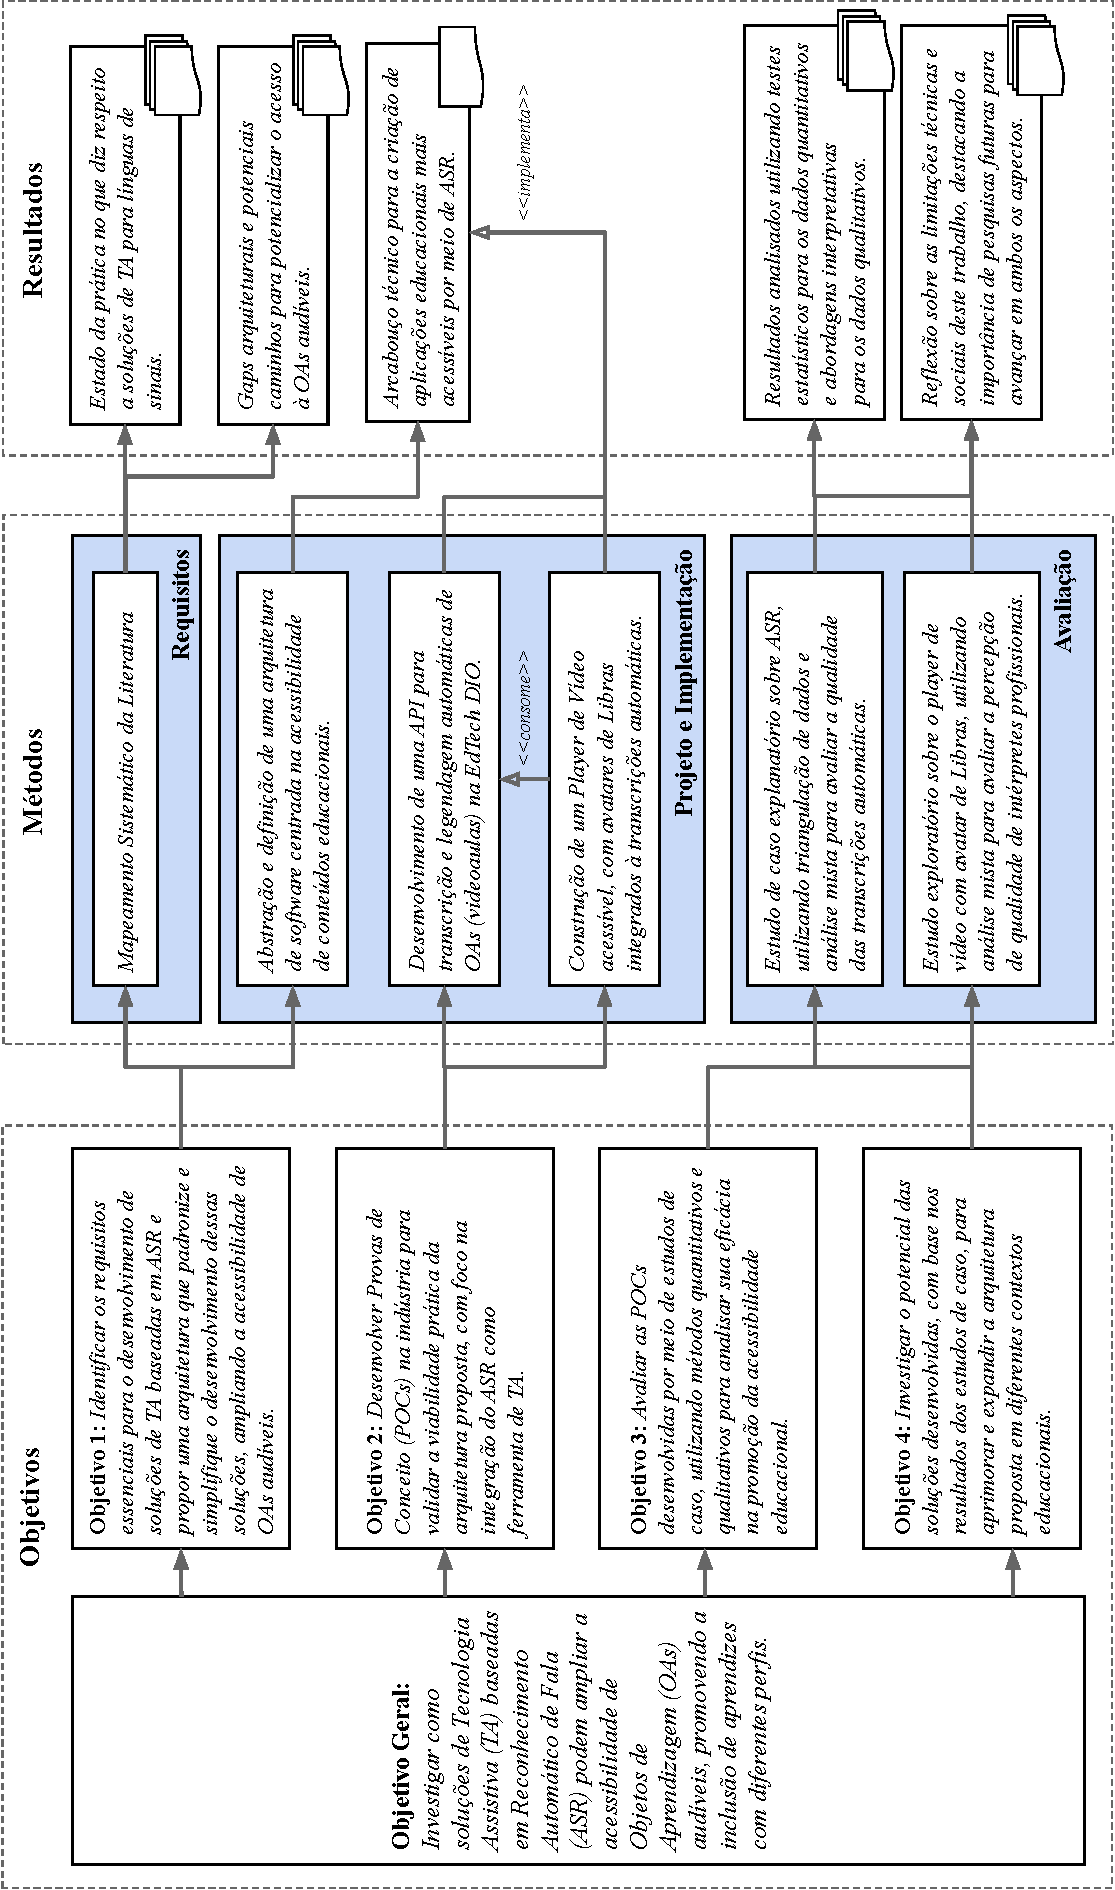
\includegraphics[width=0.85\textwidth]{images/chapter5-phd-synthesis.pdf}}
\fautor
\end{figure}

Ao longo da pesquisa, dois estudos de caso foram conduzidos para avaliar a eficácia da arquitetura em situações reais. O primeiro estudo analisou a precisão das transcrições e legendas automáticas geradas por serviços de ASR e seu impacto na acessibilidade de OAs audíveis. O segundo estudo explorou o uso de um \textit{player} de vídeo com \textit{Design} Universal, integrado tanto às transcrições automáticas quanto aos avatares de Libras, para verificar a viabilidade de uma solução mais inclusiva e multimodal.

Com base nesses estudos, esta pesquisa oferece uma série de contribuições para o campo da acessibilidade educacional, com ênfase no uso de TA para ampliar o acesso a OAs audíveis. A \autoref{chapter5-phd-synthesis}, além de ilustrar as contribuições e limitações discutidas, facilita a compreensão visual do impacto prático da pesquisa e dos desafios enfrentados ao longo dos estudos de caso. A seguir, são apresentadas as contribuições, limitações e sugestões para trabalhos futuros, destacando os avanços alcançados e as questões práticas identificadas ao longo do estudo.

\section{Contribuições da Pesquisa}

% Esta pesquisa apresentou a definição e a avaliação da arquitetura \textit{Speech2Learning}, projetada com o intuito de ampliar a acessibilidade de OAs audíveis, contribuindo para o debate sobre a inclusão educacional em diferentes contextos. A principal contribuição desta tese reside na proposição de uma abordagem que integra tecnologias de ASR para melhorar a acessibilidade educacional. As soluções desenvolvidas foram avaliadas por meio de POCs e estudos de caso, que exploraram a viabilidade prática da arquitetura em ambientes educacionais reais.

% Um dos principais achados da pesquisa foi a constatação de que os serviços de ASR, especialmente aqueles oferecidos pelos provedores OpenAI e Microsoft, demonstraram um nível de precisão elevado nas tarefas de transcrição e legendagem automática de videoaulas. Este resultado é particularmente relevante, pois confirma o potencial dessas tecnologias para contribuir de maneira significativa na acessibilidade de OAs audíveis. A precisão elevada das transcrições automáticas permite que os materiais educacionais sejam acessíveis a um público mais amplo de aprendizes, incluindo aqueles que possuem dificuldades auditivas e que dependem de legendas para compreender o conteúdo.

% Entretanto, a pesquisa também revelou limitações importantes quanto à aplicação de avatares de Libras como um recurso de TA para a comunidade surda. Apesar da integração de avatares às transcrições automáticas ter sido tecnicamente viável, os intérpretes de Libras expressaram preocupações significativas quanto à eficácia dessa abordagem. A principal crítica refere-se à complexidade inerente à Libras, que envolve nuances culturais, regionalidades e contextos que nem sempre são capturados adequadamente por avatares automatizados. Isso sugere que, embora as tecnologias de ASR possam oferecer suporte relevante, a adaptação dessas tecnologias para atender às necessidades específicas de usuários da Libras exige um aprofundamento maior e um desenvolvimento contínuo.

% Outro aspecto importante das contribuições desta pesquisa é a identificação de que nem todas as pessoas surdas ou com deficiência auditiva possuem fluência em português, o que ressalta a importância de soluções bilíngues e culturalmente sensíveis. A adoção de avatares de Libras, embora útil em determinados cenários, não substitui a necessidade de recursos mais completos e adaptáveis que respeitem a diversidade linguística e cultural da comunidade surda. Dessa forma, a pesquisa contribui para a compreensão dos desafios envolvidos na criação de soluções de TA mais inclusivas e eficazes.

% As instâncias da arquitetura \textit{Speech2Learning}, ao integrar ASR e avatares de Libras, também proporcionaram \textit{insights} valiosos sobre como essas tecnologias podem ser adaptadas para melhorar a acessibilidade educacional. A pesquisa mostrou que, enquanto o ASR pode ser altamente eficiente em fornecer transcrições precisas, a integração com avatares de Libras precisa ser repensada e aprimorada para atender às necessidades dos usuários de forma mais eficaz. A combinação dessas tecnologias em um \textit{player} de vídeo com \textit{Design} Universal, apesar das limitações destacadas pelos intérpretes nas entrevistas, oferece um modelo flexível que pode ser adaptado para diferentes contextos educacionais, destacando a potencialidade da arquitetura para ser utilizada em diversas plataformas e aplicações.

% De modo geral, esta pesquisa avançou no desenvolvimento de uma arquitetura que pode ser replicada e adaptada para diferentes contextos educacionais, promovendo a inclusão e a acessibilidade de OAs audíveis. As contribuições apresentadas nesta tese são, portanto, significativas para o campo da TA aplicada à educação, oferecendo novas perspectivas e soluções para tornar o aprendizado mais acessível e inclusivo para uma diversidade maior de aprendizes.

As contribuições desta pesquisa podem ser classificadas e detalhadas da seguinte forma, englobando os aspectos técnicos e sociais identificados durante o desenvolvimento da arquitetura proposta e a realização dos estudos:

\begin{itemize}
    \item \textbf{Desenvolvimento de uma arquitetura genérica para acessibilidade de OAs audíveis}: A pesquisa propôs uma arquitetura flexível, denominada \textit{Speech2Learning}, projetada para facilitar a integração de tecnologias de ASR e ferramentas de TA em ambientes educacionais. Essa arquitetura é suficientemente genérica para ser replicada e adaptada a diferentes contextos e perfis de aprendizes, promovendo a acessibilidade de OAs audíveis de forma ampla, sem se restringir a um público específico.

    \item \textbf{Avaliação prática e realista da arquitetura}: Dois estudos de caso foram conduzidos para avaliar a aplicabilidade da arquitetura \textit{Speech2Learning}. O primeiro estudo triangulou dados quantitativos e qualitativos, evidenciando a precisão dos serviços de ASR na transcrição automática de videoaulas e sua contribuição direta para a acessibilidade de OAs audíveis. O segundo estudo investigou o impacto de um \textit{player} de vídeo com \textit{Design} Universal, integrado tanto às transcrições automáticas quanto aos avatares de Libras, analisando a viabilidade prática e as limitações dessa abordagem multimodal.

    \item \textbf{Precisão dos serviços de ASR}: Um dos principais achados foi a constatação de que os serviços de ASR oferecidos por provedores como OpenAI e Microsoft atingem altos níveis de precisão na transcrição de conteúdos educacionais. Essa precisão é fundamental para garantir que OAs audíveis sejam acessíveis a um público mais amplo, incluindo aprendizes com deficiência auditiva que dependem de legendas ou de avatares de línguas de sinais integrados às transcrições para a compreensão do conteúdo.

    \item \textbf{Identificação de desafios na integração de avatares de Libras}: A pesquisa revelou limitações importantes na integração de avatares de Libras como ferramenta de TA. Intérpretes de Libras expressaram preocupações sobre a eficácia dos avatares automatizados em capturar a complexidade linguística e cultural da Libras, sugerindo que, embora tecnicamente viáveis, essas soluções ainda exigem melhorias substanciais para atender de forma eficaz às necessidades da comunidade surda.

    \item \textbf{Impacto de soluções sensíveis ao contexto dos aprendizes}: A pesquisa destacou a importância de soluções bilíngues e culturalmente sensíveis, considerando que nem todas as pessoas surdas ou com deficiência auditiva possuem fluência em português. A adoção de avatares de Libras, apesar de útil em determinados cenários, precisa ser complementada por recursos mais completos e adaptáveis, que respeitem a diversidade linguística e cultural da comunidade surda.

    \item \textbf{Estabelecimento de um modelo flexível para diferentes domínios educacionais}: A combinação de ASR e avatares de Libras resultou em um modelo flexível de acessibilidade educacional, que pode ser implementado em diferentes plataformas e adaptado para diversos contextos. Embora o uso de avatares ainda apresente desafios, a integração dessas tecnologias em um \textit{player} de vídeo com \textit{Design} Universal oferece uma solução promissora para aumentar a acessibilidade dos OAs em uma variedade de cenários educacionais.
\end{itemize}

\section{Limitações da Pesquisa}

Embora esta pesquisa tenha oferecido contribuições significativas, algumas limitações foram identificadas, as quais podem influenciar tanto a interpretação dos resultados quanto a condução de trabalhos futuras. A seguir, são discutidas as principais limitações identificadas:

\begin{itemize}

\item \textbf{Avaliação limitada da \textit{Speech2Learning} como um todo:} Embora a arquitetura seja a principal contribuição desta pesquisa, sua avaliação foi realizada indiretamente, por meio de duas instâncias aplicadas em estudos de caso específicos. Para uma validação arquitetural mais robusta,  trabalhos futuros poderiam explorar o uso de simulações controladas com uma maior diversidade de OAs, além de testes em ambientes educacionais com perfis de aprendizes variados. Avaliações comparativas entre instâncias da arquitetura em múltiplos cenários, considerando fatores como idioma, complexidade do conteúdo e recursos de TA utilizados, também seriam relevantes para verificar a escalabilidade e adaptabilidade da \textit{Speech2Learning}. Além disso, estudos longitudinais que acompanhem o impacto da arquitetura ao longo do tempo em cenários reais de ensino seriam úteis para compreender seu efeito contínuo na acessibilidade educacional.

\item \textbf{Evolução das soluções de ASR impulsionadas por IA:} A rapidez com que as tecnologias de ASR estão evoluindo, especialmente aquelas baseadas em IA, pode tornar os resultados desta pesquisa sobre a precisão dos provedores de ASR rapidamente obsoletos. A cada novo avanço, surgem melhorias nas capacidades de transcrição e legendagem automáticas, o que pode alterar significativamente os níveis de precisão relatados. Assim, os resultados obtidos precisam ser revisitados em estudos futuros para garantir que reflitam o estado da arte das tecnologias de ASR.

\item \textbf{Surgimento de novos provedores e modelos de ASR:} Durante o desenvolvimento desta pesquisa, novos provedores de ASR, como a NVIDIA e o Facebook, surgiram com soluções de reconhecimento de fala baseadas em seus modelos mais recentes de IAGen. Essa evolução do mercado é acompanhada por iniciativas como a plataforma HuggingFace, que promove a IA aberta e colaborativa, fornecendo um \textit{Leaderboard}\footnote{Mais informações em \url{https://huggingface.co/spaces/hf-audio/open_asr_leaderboard}} que compara o desempenho de diversos modelos oferecidos por esses e outros provedores de ASR. O surgimento de novos players e a constante atualização dos modelos destacam a necessidade de considerar esses avanços em estudos futuros, uma vez que as comparações realizadas nesta pesquisa refletem apenas os provedores disponíveis no momento da investigação.

\item \textbf{Uso de algoritmos de similaridade léxica:} A avaliação da precisão dos serviços de ASR nesta pesquisa foi realizada utilizando algoritmos de similaridade léxica que, embora adequados para o contexto estudado, podem introduzir vieses significativos. Esses algoritmos avaliam a semelhança entre transcrições geradas automaticamente e transcrições de referência, mas podem falhar em capturar nuances contextuais e variações semânticas. Como trabalhos futuros, recomenda-se a combinação desses algoritmos com outras métricas, como o WER, que é utilizado pela HuggingFace em seu \textit{Leaderboard}.

\item \textbf{\textit{Feedback} Limitado de Intérpretes de Libras:} As entrevistas realizadas com intérpretes de Libras foram limitadas, uma vez que apenas dois intérpretes participaram. A falta de um número maior de participantes dificulta uma avaliação mais ampla e robusta das percepções sobre o uso de avatares de Libras. Isso prejudica a generalização dos resultados e indica a necessidade de continuar essas entrevistas para obter uma amostra mais representativa.

\end{itemize}

As limitações apontadas ressaltam a importância de revisitar e atualizar os resultados à medida que novas tecnologias emergem e mais dados se tornam disponíveis.

\section{Trabalhos Futuros}

Com base nas limitações e nos resultados obtidos nesta pesquisa, diversas direções podem ser exploradas em trabalhos futuros. A seguir, são discutidas algumas das principais áreas que merecem atenção:

\begin{itemize}

    \item \textbf{Integração de agentes de IA na arquitetura \textit{Speech2Learning}:} Com o crescente interesse no uso de agentes inteligentes, especialmente no contexto de IAGen, uma linha de pesquisa promissora envolve a integração desses agentes na \textit{Speech2Learning}. Agentes poderiam atuar em diversas camadas da arquitetura, oferecendo suporte dinâmico e adaptativo para melhorar a acessibilidade e a personalização dos OAs. A exploração dessas diretrizes pode transformar a maneira como as diferentes camadas da arquitetura, atualmente baseadas na \textit{Clean Architecture}, são observadas e implementadas, permitindo uma evolução mais profunda e adaptativa.

    \item \textbf{Expansão das Entrevistas com Intérpretes de Libras:} Embora esta pesquisa tenha contado com a participação de dois intérpretes de Libras profissionais, é essencial ampliar esse número para garantir uma análise mais abrangente. A inclusão de mais intérpretes permitirá uma compreensão mais profunda das percepções e desafios relacionados à aplicação de avatares de Libras como solução de TA. A ampliação desse conjunto de dados possibilitará uma avaliação mais robusta, contribuindo para melhorias e adaptações mais eficazes nas soluções desenvolvidas.

    \item \textbf{Integração com Repositórios de OAs:} Um aspecto relevante para o sucesso da arquitetura \textit{Speech2Learning} é a facilidade com que os OAs podem ser integrados e disponibilizados através da arquitetura proposta. Trabalhos futuros devem focar em simplificar essa integração, criando métodos mais naturais e eficientes para o acoplamento de OAs com a \textit{Speech2Learning}. Isso inclui o desenvolvimento de APIs e conectores que facilitem a disponibilização dos OAs de forma automática e intuitiva, reduzindo a necessidade de intervenções manuais.

    \item \textbf{Melhorias no \textit{Player} de Vídeo com \textit{Design} Acessível:} Baseado nos \textit{feedbacks} recebidos durante esta pesquisa, trabalhos futuros devem focar em aprimorar tecnicamente o \textit{player} de vídeo desenvolvido. Isso inclui não apenas a integração mais fluida com avatares de Libras, mas também melhorias gerais na usabilidade e acessibilidade do \textit{player}. A realização de testes de usabilidade, baseados em heurísticas como as de Nielsen, pode fornecer percepções valiosas para aperfeiçoar a experiência do usuário. Além disso, a disponibilização do \textit{player} como uma biblioteca \textit{open-source} permitirá que a comunidade contribua com seu desenvolvimento e expansão.

    \item \textbf{Documentação e Atualização da \textit{Speech2Learning}:} Embora a evolução das tecnologias de ASR não afete diretamente a \textit{Speech2Learning}, é crucial que a documentação e as definições da arquitetura acompanhem essas evoluções. Isso garantirá que a \textit{Speech2Learning} continue a ser uma ferramenta relevante, mesmo com o surgimento de novas tecnologias e metodologias. A documentação deve ser revisada e atualizada periodicamente para incorporar as melhores práticas e garantir a compatibilidade com os avanços tecnológicos.

\end{itemize}

Essas direções apontam para a necessidade de continuar a evolução da \textit{Speech2Learning} e suas aplicações, garantindo que a arquitetura se mantenha adaptável e relevante em um cenário educacional em constante transformação.

\section{Publicações Resultantes}

As principais publicações resultantes das atividades conduzidas nesta pesquisa de doutorado são apresentadas a seguir, ordenadas cronologicamente:

\begin{enumerate}
    
    \item \citeonline{FalvoJr2020_SBIE}: \fullcite{FALVOJR, V.; MARTINS FALVO, C.; SCATALON, L.; BARBOSA, E.}{Tecnologias Aplicadas ao Ensino e Aprendizagem de LIBRAS: Um Mapeamento Sistemático}{Simpósio Brasileiro de Informática na Educação (SBIE)}{2020}{Disponível em \url{doi.org/10.5753/cbie.sbie.2020.812}}

    \item \citeonline{FalvoJr2020_FIE}: \fullcite{FALVOJR, V.; SCATALON, L.; BARBOSA, E.}{The Role of Technology to Teaching and Learning Sign Languages: A Systematic Mapping}{Frontiers in Education Conference (FIE)}{2020}{Disponível em \url{doi.org/10.1109/FIE44824.2020.9274169}}

    \item \citeonline{FalvoJr2021_RENOTE}: \fullcite{FALVOJR, V.; MARTINS FALVO, C.; SCATALON, L.; BARBOSA, E.}{Tecnologias Aplicadas ao Ensino e Aprendizagem com Línguas de Sinais: Um Mapeamento Sistemático Sob as Perspectivas Nacional e Internacional}{Revista Novas Tecnologias na Educação (RENOTE)}{2021}{Disponível em \url{doi.org/10.22456/1679-1916.110217}}

    \item \citeonline{FalvoJr2023_HICSS}: \fullcite{FALVOJR, V.; MARCOLINO, A.; BRUNO, D.; MARTINS FALVO, C.; OSÓRIO, F.; BARBOSA, E.}{Lexical Analysis of Automatic Transcriptions Using Speech-to-Text Services: A Statistically Evaluated Case Study}{Hawaii International Conference on System Sciences (HICSS)}{2024}{Disponível em \url{hdl.handle.net/10125/107023}}

    \item \citeonline{FalvoJr2024_FIE}: \fullcite{FALVOJR, V.; MARCOLINO, A.; BRUNO, D.; MARTINS FALVO, C.; OSÓRIO, F.; BARBOSA, E.}{Enhancing Learning Objects Accessibility Through Speech-To-Text Based Architecture: A Comprehensive Triangulation Study}{Frontiers in Education (FIE)}{2024}{Submetido em 20/05/2024 e aceito em 23/07/2024}
\end{enumerate}

De modo complementar, outros trabalhos indiretamente relacionados a esta pesquisa também foram publicados. Esta colaboração contínua entre pesquisadores, muitas vezes de diferentes instituições, propiciou descobertas e percepções fundamentais para a idealização e desenvolvimento deste trabalho de doutorado \cite{Soad2017_FIE,Oliveira2019_SBIE,FalvoJr2022_JUCS,FalvoJr2023_SMarty}:

\begin{enumerate}\setcounter{enumi}{4}
    
    \item \citeonline{Soad2017_FIE}: \fullcite{SOAD, G.; FIORAVANTI, M.; FALVOJR, V.; MARCOLINO, A.; DUARTE FILHO, N.; BARBOSA, E.}{ReqML-catalog: The Road to a Requirements Catalog for Mobile Learning Applications}{Frontiers in Education Conference (FIE)}{2017}{Disponível em \url{doi.org/10.1109/FIE.2017.8190718}}
    
    \item \citeonline{Oliveira2019_SBIE}: \fullcite{OLIVEIRA, R.; FALVOJR, V.; BARBOSA, E. F.}{Internet das Coisas aplicada à Educação: Um Mapeamento Sistemático}{Simpósio Brasileiro de Informática na Educação (SBIE)}{2019}{Disponível em \url{doi.org/10.5753/cbie.sbie.2019.499}}
    
    \item \citeonline{FalvoJr2022_JUCS}: \fullcite{FALVOJR, V.; MARCOLINO, A.; DUARTE FILHO, N.; OLIVEIRAJR, E.; BARBOSA, E.}{Variability-based Improvement of M-Learning Applications Development}{Journal of Universal Computer Science (J.UCS)}{2022}{Disponível em \url{doi.org/10.3897/jucs.90663}}
    
    \item \citeonline{FalvoJr2023_SMarty}: \fullcite{FALVOJR, V.; MARCOLINO, A.; DUARTE FILHO, N.; OLIVEIRAJR, E.; BARBOSA, E.}{A Software Product Line for Mobile Learning Applications}{Capítulo 13 do Livro ``UML-Based Software Product Line Engineering with SMarty''}{2023}{Disponível em \url{doi.org/10.1007/978-3-031-18556-4_13}}
\end{enumerate}
